\begin{figure}[H]
\centering
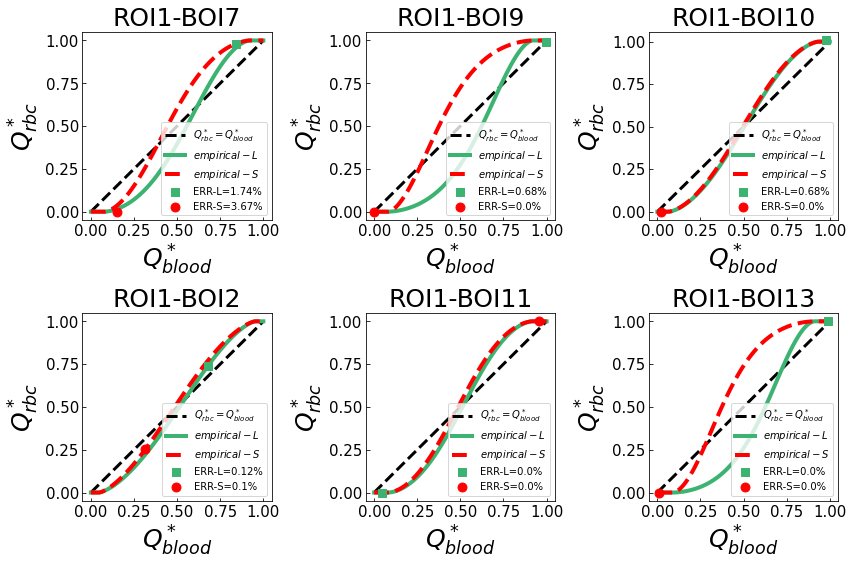
\includegraphics[width=0.775\textwidth]{images/DisproportionalityIndexQblood-ROI1.png}
\caption{\textit{Deviations between simulation data (squares/circle) and empirical predictions (solid lines) from PSM expressed as fractional RBC flux (Q$^{*}_{rbc}$) against fractional blood flow (Q$^{*}_{blood}$) for all selected diverging bifurcation within ROI-1. (see Figure \ref{ROIs}a) For each bifurcation, the "L" and "S" terms indicate the relatively larger (green coloured) and smaller (red coloured) child branches respectively. The black dotted line represents the linear theoretical line for Q$^{*}_{blood}$ and Q$^{*}_{rbc}$ without the presence of plasma skimming.} \label{DisproportionalityIndexQblood-ROI1}}
\end{figure}


\useportrait
\begin{figure}[H]
\centering
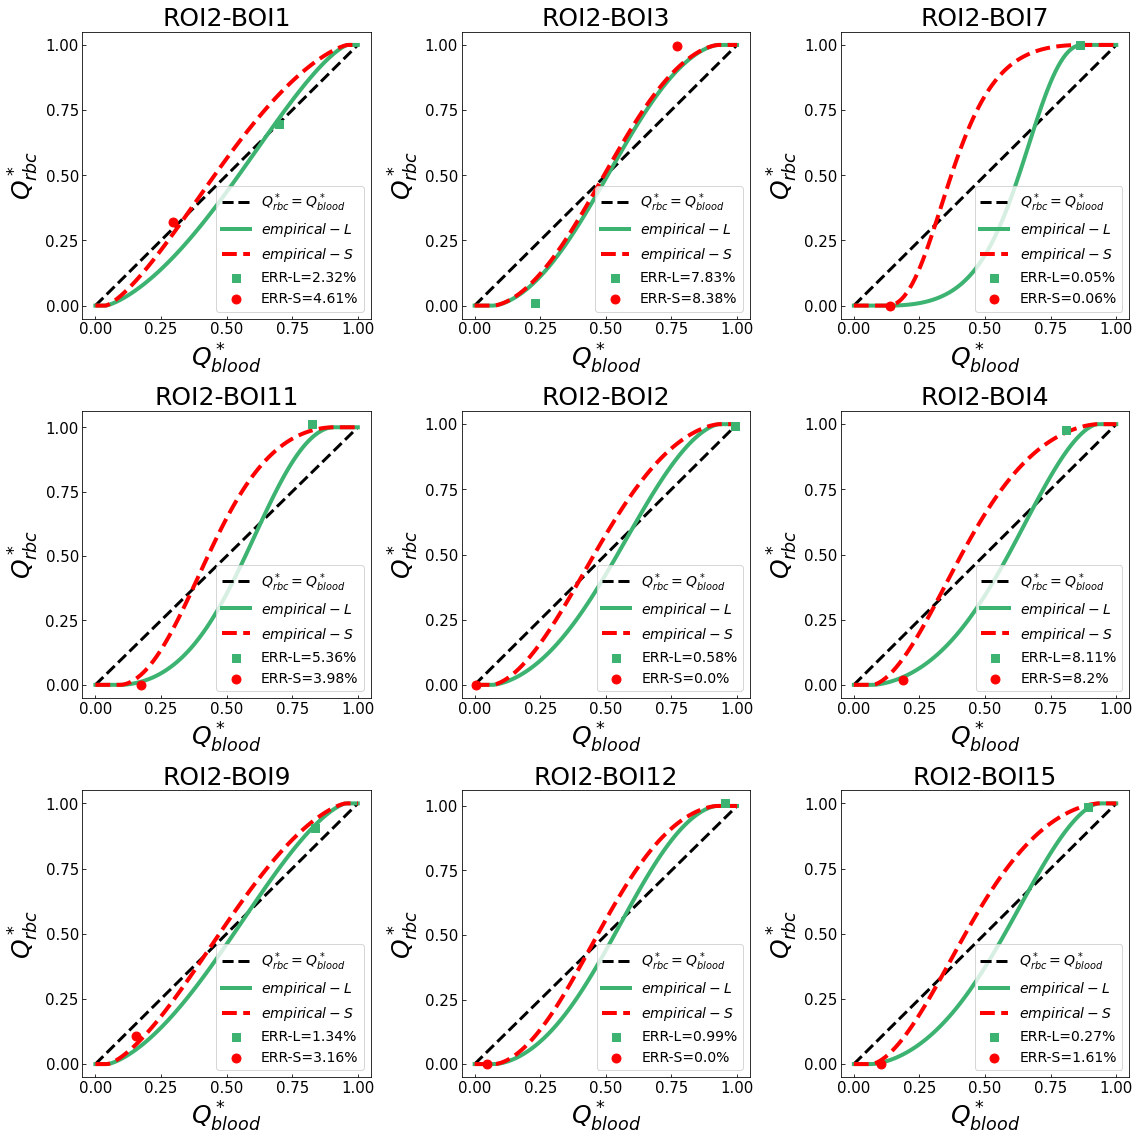
\includegraphics[width=1\textwidth]{images/DisproportionalityIndexQblood-ROI2.png}
\caption{\textit{Deviations between simulation data (squares/circle) and empirical predictions (solid lines) from PSM expressed as fractional RBC flux (Q$^{*}_{rbc}$) against fractional blood flow (Q$^{*}_{blood}$) for all selected diverging bifurcation within ROI-2. (see Figure \ref{ROIs}b) For each bifurcation, the "L" and "S" terms indicate the relatively larger (green coloured) and smaller (red coloured) child branches respectively. The black dotted line represents the linear theoretical line for Q$^{*}_{blood}$ and Q$^{*}_{rbc}$ without the presence of plasma skimming.} \label{DisproportionalityIndexQblood-ROI2}}
\end{figure}


\uselandscape
\begin{figure}[H]
\centering
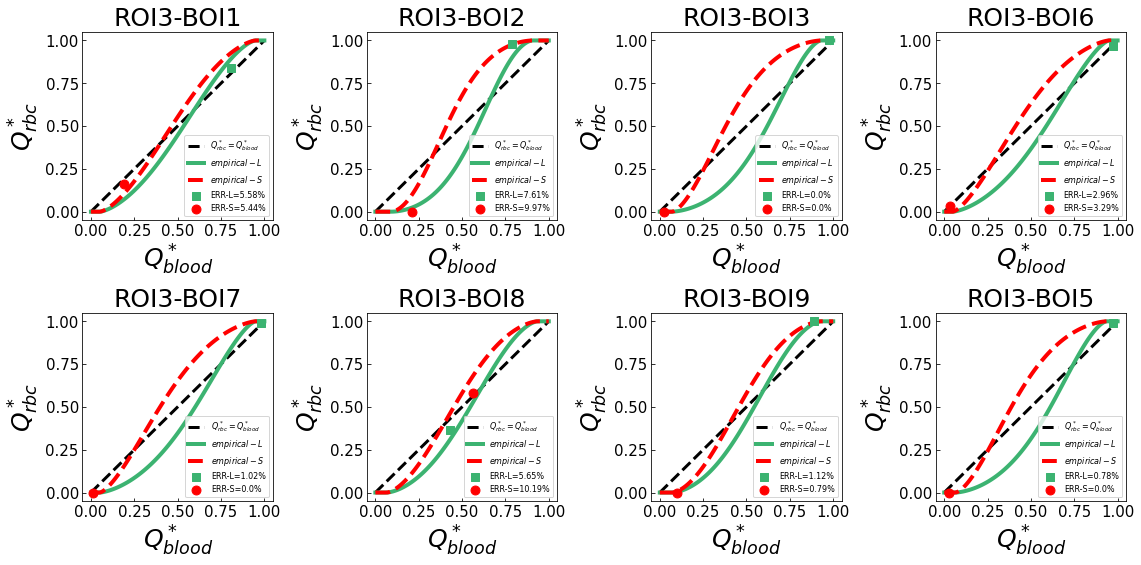
\includegraphics[width=1\textwidth]{images/DisproportionalityIndexQblood-ROI3.png}
\caption{\textit{Deviations between simulation data (squares/circle) and empirical predictions (solid lines) from PSM expressed as fractional RBC flux (Q$^{*}_{rbc}$) against fractional blood flow (Q$^{*}_{blood}$) for all selected diverging bifurcation within ROI-3. (see Figure \ref{ROIs}c) For each bifurcation, the "L" and "S" terms indicate the relatively larger (green coloured) and smaller (red coloured) child branches respectively. The black dotted line represents the linear theoretical line for Q$^{*}_{blood}$ and Q$^{*}_{rbc}$ without the presence of plasma skimming.} \label{DisproportionalityIndexQblood-ROI3}}
\end{figure}